\newpage
\section{Functional requirements}

% reviewing of the cases by another caseworker before processing the loss of earnings. 
% funtionelle ting som er målbare!!!!
The applicant is required to login to the OCM system as a citizen to access application form. Applicant fill in data into application form and attach any additional documentation. To submit the application, the applicant needs press submit button and confirm the submission on subsequent confirmation.

\vspace{2mm}

The OCM system checks for existing applications from applicant. If none are found the system annotate the case as new, otherwise it annotate the case as duplicate. The system sends application to a random caseworker.

\vspace{2mm}

The caseworker is required to login to the OCM system as a caseworker. The caseworker can make an overview of all unprocessed cases, approval cases and ongoing cases that is assigned to the caseworker. Caseworker takes an unprocessed case, approval case or pick one of his existing cases that is ongoing.

If the caseworker takes an unprocessed case, the person will be presented with all the provided documents from the applicant. If the caseworker decides the documents are falsified, he changes the status to falsified and either gets unassigned from the case or takes further action by contacting the legal authorities and provide all the necessary information, that is requested. After the falsification is handled, the case change status to prosecuted.

After the verification of the authenticity of the documents, the caseworker decides if the doctor confirmation is confirming that the legal requirements of the child's health status is met and the necessary conditions are present. 
If the conditions are not met, the application gets rejected. 
If the documents provided does not fulfill the necessary conditions, the caseworker can send an email directly from the system to the applicant, requesting the necessary documents for further processing of the application.

When satisfactory is met and all the conditions and legal documents are met, the caseworker goes on to verify that the inputted numbers are correct.

If the caseworker picks an approval case, that is not handled by the caseworker himself. The caseworker goes through all documents provided and verifies that the applicant is permitted for loss of earnings. The caseworker goes on to verify that the inputted numbers are correct.
If the caseworker decides, that the applicant is not permitted for loss of earnings, the caseworker sets the case to rejected.

If the caseworker decides, that the applicant is permitted for loss of earning, the caseworker sets the case to approved.

---

The applicant is presented with a form, that contains all the required input fields and required fields for document upload. After submitting the application the applicant will receive an email from the system confirming the submission.

If the application needs some information, the applicant would receive a request per email and a link to the formula with the information that is previously provided. The application now has the possibility to input the requested information. 

If the application is rejected, the applicant receives cause of rejection per email.

If the application is approved, the applicant receives the acceptance confirmation per email. 

---

If the application is rejected or accepted twice, the system would send the decision to the applicant and archive the case. 

---

The supervisor can make an overview of all open cases and all archived cases. The supervisor can inspect the current information that belongs to a case and what caseworker it is assigned to.

\begin{figure}[htb!]
	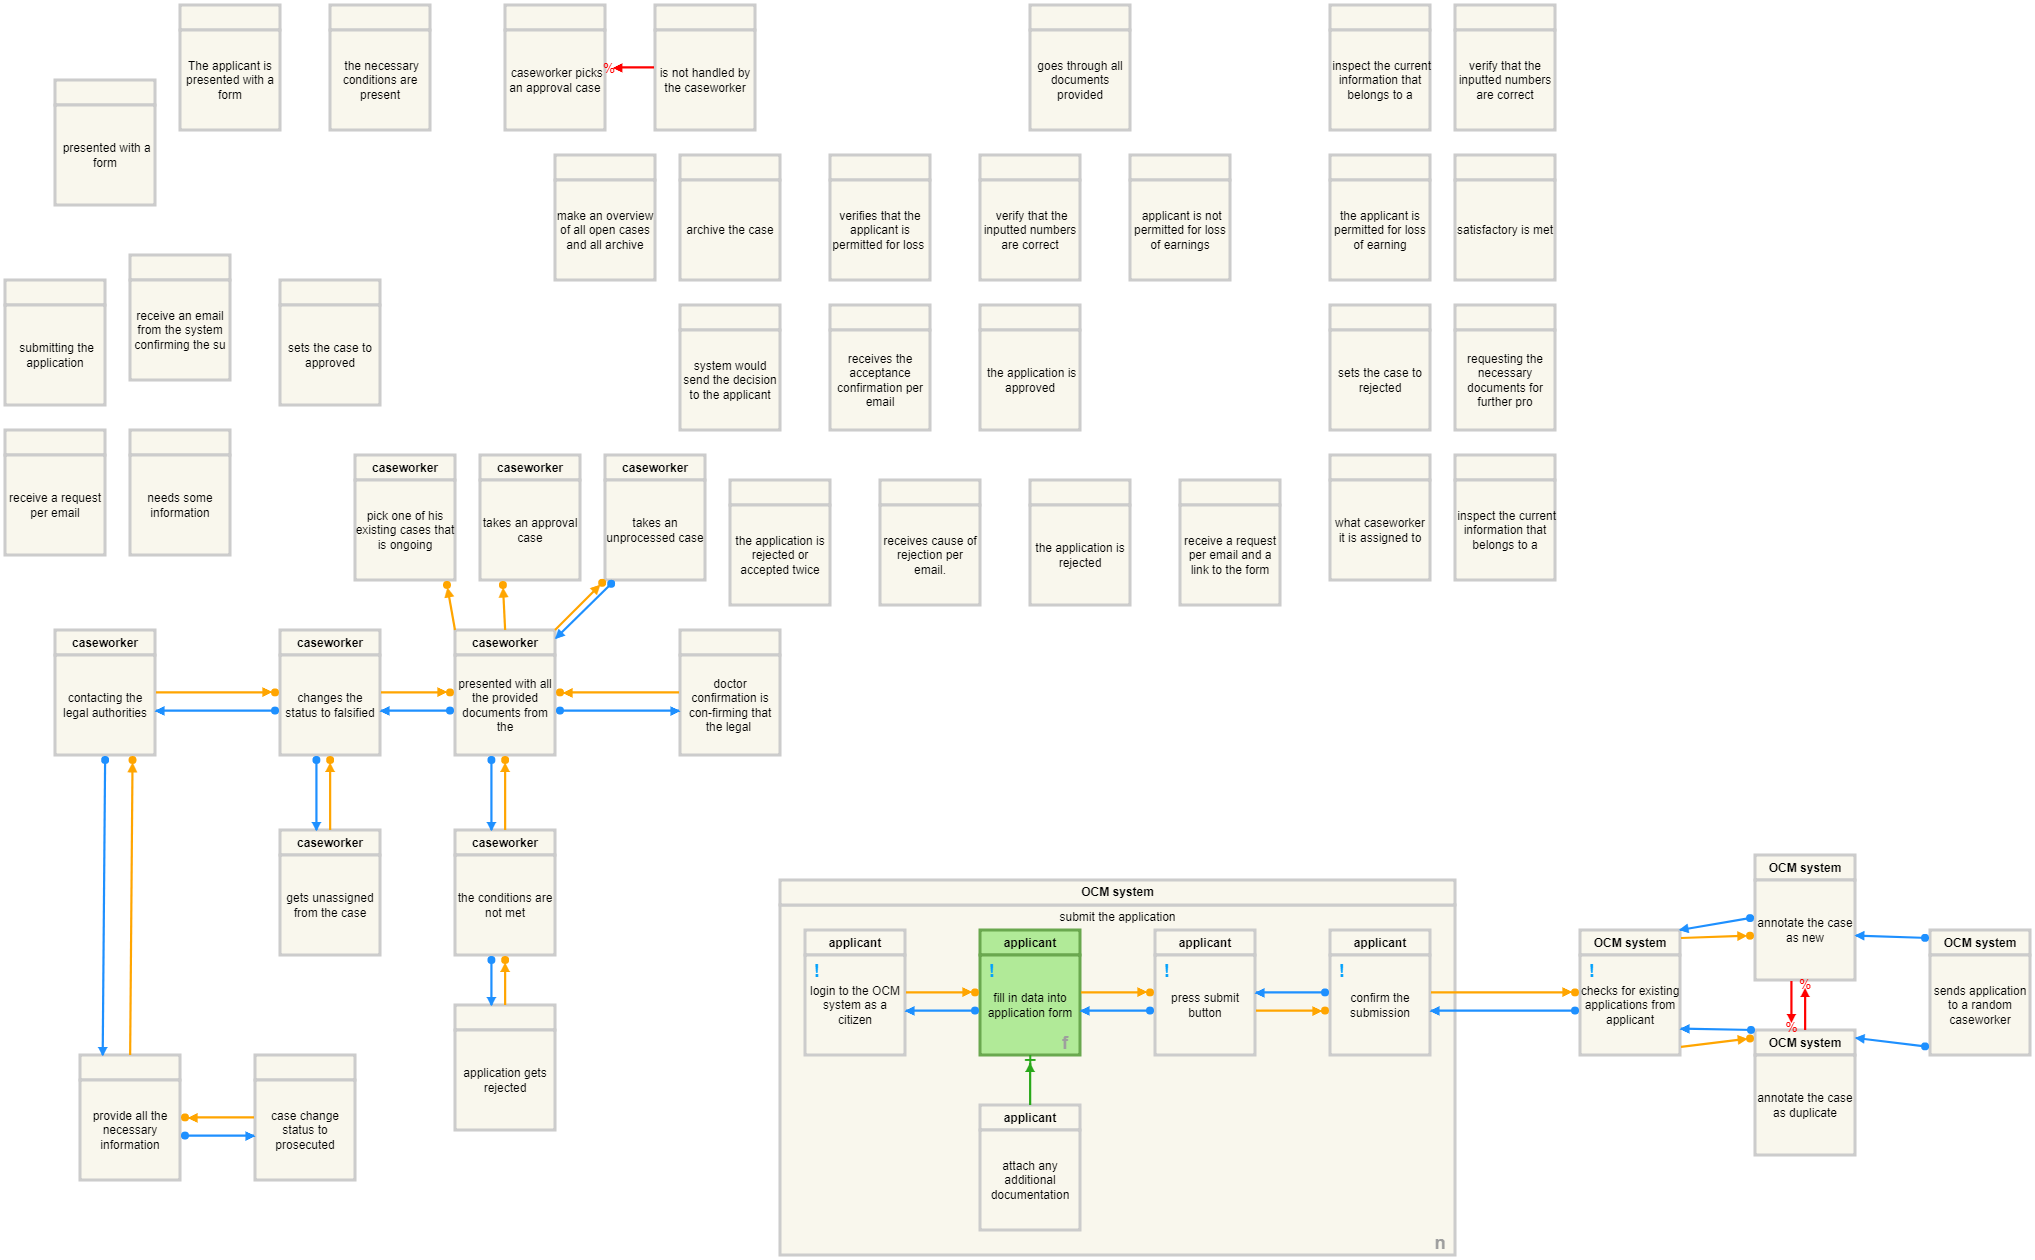
\includegraphics[width=\textwidth]{img/dcr}
	\caption{A very rough dcr graph}
\end{figure}